%----------------------------------------------------------------------------------------
%	%PACKAGES, THEMES and COMMANDS
%----------------------------------------------------------------------------------------

\documentclass[aspectratio=169,xcolor=dvipsnames]{beamer}
\usetheme{Boadilla}
\usecolortheme{dolphin}
\setbeamertemplate{caption}[numbered]
\usepackage{amsmath}
\usepackage{mathtools}
\usepackage{hyperref}
\usepackage{tikz}
\usetikzlibrary {arrows.meta}
\usepackage{hyperref}
\usepackage[authoryear, round]{natbib}
\usepackage{algorithm,algorithmic}
\DeclareMathOperator{\R}{\mathbb{R}}
\newcommand*\diff{\mathop{}\!\mathrm{d}}
\newcommand{\blue}{\color{myblue}}
\newcommand{\red}{\color{red}}
\newcommand{\green}{\color{ForestGreen}}
\newcommand{\black}{\color{black}}
\newcommand{\di}{\text{d}}
\newcommand{\vecx}{\textbf{x}}
\newcommand{\vecpi}{\boldsymbol{\pi}}
\newcommand{\vecc}{\textbf{c}}
\newcommand{\vecz}{\textbf{z}}
\newcommand{\matx}{\textbf{X}}
\newcommand{\matz}{\textbf{Z}}
\newcommand{\aOverK}{\frac{\alpha}{K}}
\definecolor{myblue}{RGB}{60,60,200}

%----------------------------------------------------------------------------------------

\title[IBP, Griffiths and Ghahramani]{The Indian Buffet Process: An Introduction and Review
} \subtitle{T. L. Griffiths, and Z. Ghahramani, 2001.}
\author[andrea.teruzzi@proton.me] {Andrea Teruzzi}
\date[VSI – BayesLab]{November 25, 2022} 

%----------------------------------------------------------------------------------------
%----------------------------------------------------------------------------------------

\begin{document}
\begin{frame}
    \titlepage
\end{frame}
  \begin{frame}
    \frametitle{Table of Contents}
    \tableofcontents
  \end{frame}

%---------------------------------------------------------------------------------------

%---------------------------------------------------------------------------------------
\section{Introduction} 
\begin{frame}{Introduction - Latent Structure Problem}
\setlength{\leftmargini}{0.2cm}
\begin{itemize}
    \item One key goal of unsupervised learning is to determine the amount of \textbf{latent structure} associated to each data object.
    \begin{itemize}
        \item Cluster assignment
        \item Number of features 
    \end{itemize}
    \item The alternative is to assume that the amount of latent structure is \textbf{unbounded} 
    \begin{itemize}
        \item \textbf{Bayesian non-parametric} (BNP) methods are extremely suited for this scope
        \item The celebrated \textbf{Dirichlet process mixture} (DPM) , is a good example of unbounded number of latent components. 
    \end{itemize}
    \item In DPM \textbf{each datapoint is assigned to latent class} and each class is associated with a distribution. The particular feature of the model is that the prior responsible of assigning observations to latent class is bounded only by the number of objects, making DPM models \textbf{“infinite” mixture models}.
    \begin{itemize}
        \item Generative process: \textbf{Chinese restaurant process}
    \end{itemize}
\end{itemize}
\end{frame}
%---------------------------------------------------------------------------------------
\begin{frame}{Introduction – Beyond the DPM}
\setlength{\leftmargini}{0.2cm}
\begin{itemize}
    \item DPM has been subject to several extensions, but all of this models associate each object with \textbf{one latent variable} that assigns the object to one class or parameter determining its probability law.
    \begin{itemize}
        \item That is not always the case! As each object can be produced by \textbf{multiple (unknown) number of causes} and presenting multiple feature.
    \end{itemize}
    \item We can \textbf{represent each object with a binary vector}, with entries indicating the presence or absence of each feature.
    \begin{itemize}
        \item We would like to not put an upper bound to the number of features. Dirichlet process are not suited for this goal.
    \end{itemize}
    \item The objective of the paper is presenting a non-parametric approach to models in which objects are represented using an unknown number of latent feature.
    \begin{itemize}
        \item Generative process: \textbf{Indian buffet process}
    \end{itemize}
\end{itemize}
\end{frame}
%---------------------------------------------------------------------------------------
%---------------------------------------------------------------------------------------

\section{Latent Class Models} 
\subsection{Finite Latent Class Models} 
\begin{frame}{Latent Class Models}
\setlength{\leftmargini}{0.2cm}
\begin{itemize}
\item Assume we have $N$ row vectors (objects) $\vecx_i$ each having $D$ observable properties and the matrix $\matx = [\vecx^{\top}_1 \vecx^{\top}_2 \dots \vecx^{\top}_N ]$ to indicate the properties of all the objects.
\item We assign each $\vecx_i$ to a single class $c_i$ and we indicate with $\vecc$ the class assignment of each object.
\item The statistical model for a latent class model consists in specifying 
\begin{gather*}
  P(\vecc) \\
  p(\matx|\vecc)   
\end{gather*}
\end{itemize}
\end{frame}
%---------------------------------------------------------------------------------------
\begin{frame}{Finite Mixture Model}
\setlength{\leftmargini}{0.2cm}
\begin{itemize}
\item Mixture models assume that \textbf{the assignment of an object to a class is independent of the assignments of all other objects}. In finite mixture model we have $K$ classes.
\begin{align*}
    P(\vecc) &= \prod_{i=1}^{N} P(c_i| \, \theta) =  \prod_{i=1}^{N} \theta_{c_i},
\end{align*}
with $\theta$ multinomial distribution and $\theta_k$ the probability of class k under that distribution (i.e. $\sum_{k=1}^{K} \theta_k=1$)
\item Under this assumption:
\begin{equation*}
      p(\matx|\vecc) = \prod_{i=1}^{N} \sum_{k=1}^{K} p(\vecx_i| \, c_i=k)\theta_k,
\end{equation*}
that is a mixture of the $K$ class distributions $p(\vecx_i| \, c_i = k)$, with $\theta_k$ determining the weight of class $k$.
\end{itemize}
\end{frame}
%---------------------------------------------------------------------------------------
\begin{frame}{Finite Mixture Model}
\setlength{\leftmargini}{0.2cm}
\begin{itemize}
\item In Bayesian modeling, $\theta$ is assumed to follow a prior distribution $p(\theta)$, with conjugate choice the \textbf{Dirichlet distribution over K classes} with parameters $\alpha_1,\alpha_2,\dots,\alpha_K$.
\begin{equation*}
    p(\theta) = \frac{\prod_{k=1}^{K}\theta^{\alpha_k-1}_{k}}{D(\alpha_1,\alpha_2,\dots,\alpha_K)},
\end{equation*}
with normalizing constant $D(\alpha_1,\alpha_2,\dots,\alpha_K)$ define as
\begin{align*}
    D(\alpha_1,\alpha_2,\dots,\alpha_K) &= \int_{\Delta_{K}} \prod_{k=1}^{K}\theta^{\alpha_k-1}_{k} \diff \theta \\ &= \frac{\prod_{k=1}^{K} \Gamma(\alpha_{k})}{\Gamma(\sum_{k=1}^{K}\alpha_{k})},
\end{align*}
where $\Delta_K$ is the simplex of multinomials over $K$ classes  and $\Gamma(m) = (m - 1)!$ is the gamma function.
\end{itemize}
\end{frame}
%---------------------------------------------------------------------------------------
\begin{frame}{Finite Mixture Model}
\setlength{\leftmargini}{0.2cm}
\begin{itemize}
\item Using a symmetric Dirichlet (i.e. $\alpha_k = \aOverK$ for all $k$):
\begin{align*}
    \theta | \, \alpha &\sim \text{Dirichlet}\Big(\aOverK, \aOverK, \dots, \aOverK\Big) \\ c_i | \theta & \sim \text{Discrete}(\theta),
\end{align*}
where $\text{Discrete}(\theta)$ is the multiple-outcome analogue of a Bernoulli event, where the probabilities of the outcomes are specified by $\theta$.
\end{itemize}
\vspace{1pt}
\begin{figure}
\begin{center} 
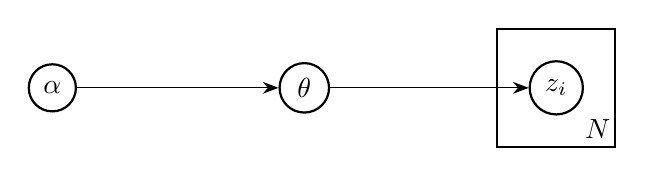
\begin{tikzpicture} [scale = 1.6] 
        %style
        \tikzset{circle/.style = {shape=circle, draw ,minimum size=1.5em, text opacity=1, thick}}
        \tikzset{rectangle/.style = {shape=rectangle, draw, minimum size=1.5,text opacity=1, thick, minimum width = 1.5cm, minimum height = 1.5cm}}
        \node[circle]    (alpha) at  (0,0) {$\alpha$};
        \node[circle]    (theta) at  (2,0) {$\theta$};
        \node[circle]    (zeta)  at  (4,0) {$z_i$};
        \node[rectangle] (quad)  at  (4,0) {};
        \node            (N)     at  (4.33,-0.33) {$N$};
        \draw [-{Stealth[length=2mm]}] (alpha) to (theta);
        \draw [-{Stealth[length=2mm]}] (theta) to (zeta);
\end{tikzpicture}
\caption{Graphical model for the Dirichlet-multinomial model}
\label{fig:dirichlet_mult}
\end{center}
\end{figure}
\end{frame}
%---------------------------------------------------------------------------------------
\begin{frame}{Finite Mixture Model}
\setlength{\leftmargini}{0.2cm}
\begin{itemize}
\item Integrating over all values of $\theta$ the probability of an assignment vector $\vecc$ is:
\begin{align}
    P(\vecc) = \int_{\Delta_{K}} \prod_{i=1}^{n} P(c_i| \theta) p(\theta) \diff \theta 
    &= \int_{\Delta_{K}} \frac{\prod_{k=1}^{K}\theta^{m_k + \alpha/K-1}_{k}}{D(\aOverK,\aOverK,\dots,\aOverK)} \diff \theta  \nonumber \\
    &= \frac{D(m_1+\aOverK, m_2+\aOverK,\dots, m_k +\aOverK)}{D(\aOverK,\aOverK,\dots,\aOverK)}  \nonumber\\
    &= \frac{\prod_{k=1}^{K} \Gamma(m_k + \aOverK )}{\Gamma(\aOverK)^{K}} \frac{\Gamma(\alpha)}{\Gamma(N+\alpha)},  \label{eq:dir_mu}
\end{align} 
where $m_k=\sum_{i=1}^{N}\delta(c_i=k)$ is the number of objects assigned to class k.
\item Class assignments $\vecc$ are not independent, rather they are \textbf{exchangeable}.
\item Equation \ref{eq:dir_mu} \textbf{assumes an upper bound on the number of classes} of objects
\end{itemize}
\end{frame}
%---------------------------------------------------------------------------------------
\begin{frame}{Infinite Mixture Models}
\setlength{\leftmargini}{0.2cm}
\begin{itemize} 
\item We specify the probability of $\matx$ for infinitely many classes:
\begin{equation*}
      p(\matx|\vecc) = \prod_{i=1}^{N} \sum_{k=1}^{\infty} p(\vecx_i| \, c_i=k)\theta_k
\end{equation*}
\begin{enumerate}
    \item Define a prior $p(\theta)$ on infinite-dimensional multinomials and compute $p(c)$ by integrating over $\theta$
    \item Consider Equation \ref{eq:dir_mu} and take the limit for $K\rightarrow\infty$
\end{enumerate}
\item We rearrange Equation \ref{eq:dir_mu} considering the recursion property of $\Gamma(x)$:
\begin{equation}
    P(\vecc) = \Big(\aOverK\Big)^{K_+} \bigg( \prod_{k=1}^{K_{+}} \prod_{j=1}^{m_k-1}\Big(j+\aOverK\Big) \bigg) \frac{\Gamma(\alpha)}{\Gamma(N+\alpha)},  \label{eq:pr_c_lim}
\end{equation}
with $K_+$ is the number of classes for which $m_k > 0$ for the ordered sequence
of indices such that $m_k > 0$ for all $k <K_+$.
\item Since there are $K^N$ possible configurations for $\vecc$, $P(\vecc) \rightarrow 0$ as $K \rightarrow \infty$.
\end{itemize}
\end{frame}
%---------------------------------------------------------------------------------------
\begin{frame}{Distribution over partitions}
\setlength{\leftmargini}{0.2cm}
\begin{block}{Definition}
A \textbf{partition} is a division of the set of $N$ objects into subsets, where each object belongs to a single subset and the ordering of the subsets does not matter.
\end{block}
\begin{equation*}
    e.g. \quad \{c_1, c_2, c_3\} = \{1, 1, 2\} \text{ is equivalent to } \{2, 2, 1\}
\end{equation*}
\begin{itemize} 
\item A partition defines an \textbf{equivalence class} of assignment vectors, which we denote $[\vecc]$
\item $p(\matx |\,\vecc)$ is the same for all vectors $\vecc$ corresponding to the same partition $[\vecc]$
\item Assume we have a partition of $N$ objects into $K_+$ subsets with $K = K_0 + K_+$ classes. There are $\frac{K!}{K_0}$ assignments of vector $\vecc$ that belong to the equivalence class defined by that partition  $[\vecc]$

\end{itemize}  
\end{frame}
%---------------------------------------------------------------------------------------
\subsection{Infinite Mixture Models}
\begin{frame}{Distribution over partitions}
\setlength{\leftmargini}{0.2cm}
\begin{itemize} 
\item The limiting probability of those class assignments is:
\begin{align}
    P([\vecc]) = \sum_{\vecc\in[\vecc]}P(\vecc) &= \lim_{K\rightarrow\infty} \frac{K!}{K_0!}P(\vecc) \nonumber \\
    &=\lim_{k\rightarrow\infty} \frac{K!}{K_0!} \Big(\aOverK\Big)^{K_+} \bigg( \prod_{k=1}^{K_{+}} \prod_{j=1}^{m_k-1}\Big(j+\aOverK\Big) \bigg) \frac{\Gamma(\alpha)}{\Gamma(N+\alpha)} \nonumber \\
    &=  \alpha^{K^+} \bigg( \prod_{k=1}^{K_{+}}\Big(m_k - 1\Big)! \bigg) \frac{\Gamma(\alpha)}{\Gamma(N+\alpha)}, \label{eq:limit_partition}
\end{align}
that defines a \textbf{distribution over partitions} that is the prior over class assignments for an infinite mixture model.
\item Equation \ref{eq:limit_partition} is consistent with the other derivation, as Dirichlet Process \citep{blackwel_mcq_73} or stick breaking priors \citep{sethuraman94}.
\end{itemize}  
\end{frame}
%---------------------------------------------------------------------------------------
\subsection{The Chinese Restaurant Process}
\begin{frame}{The Chinese Restaurant Process}
Imagine a restaurant with an infinite number of tables, each with an infinite number of seats. The $i$th client will seat to the $k$th table with probability:
\begin{equation*}
    P(c_i = k|c_1, c_2, \dots, c_{i-1})  =\begin{cases}
        \frac{m_k}{i-1+\alpha} \quad k\leq K_+\\
        \frac{\alpha}{i-1+\alpha} \quad k = K + 1
    \end{cases}
\end{equation*}
\onslide<2->{
\begin{figure}
\begin{center} 
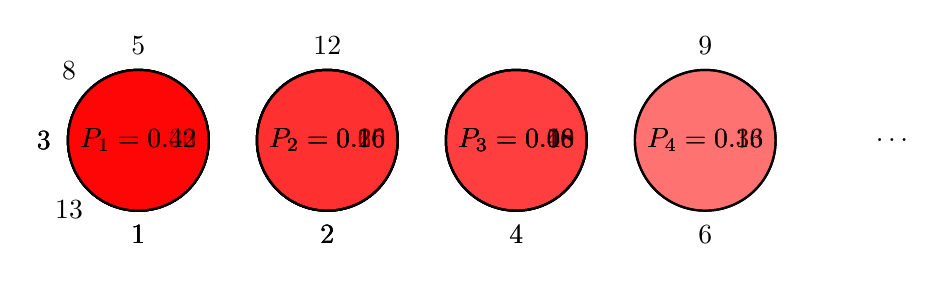
\begin{tikzpicture} [scale = 1.6] 
        %style
        \tikzset{circle/.style = {shape=circle, draw ,minimum size=1.7cm, text opacity=1, thick, fill=red}}
        \tikzset{no_circle/.style = {shape=circle, draw ,minimum size=1.7cm, text opacity=1, thick, white, fill= white, fill opacity=0.2}}
        \onslide<2>{
        \node[circle, fill opacity=0.75]    (tab1) at  (0.0,0.0) {$P_1=1.00$};
        \node[no_circle]    (tab2) at  (1.5,0.0) {$P_2=0.00$};
        \node[no_circle]    (tab3) at  (3.0,0.0) {$P_3=0.00$};
        \node[no_circle]    (tab4) at  (4.5,0.0) {$P_4=0.00$};
        \node[white]            (dots) at  (6.0,0.0) {$\dots$};
        }
        \onslide<3>{
        \node[circle, fill opacity=0.25]    (tab1) at  (0.0,0.0) {$P_1=0.33$};
        \node[circle, fill opacity=0.50]    (tab2) at  (1.5,0.0) {$P_2=0.66$};
        \node[no_circle]    (tab3) at  (3.0,0.0) {$P_3=0.00$};
        \node[no_circle]    (tab4) at  (4.5,0.0) {$P_4=0.00$};
        \node[white]     (dots) at  (6.0,0.0) {$\dots$};
        \node             (N)    at  (0.0,-0.75) {$1$};
        }
        \onslide<4>{
        \node[circle, fill opacity=0.20]    (tab1) at  (0.0,0.0) {$P_1=0.25$};
        \node[circle, fill opacity=0.20]    (tab2) at  (1.5,0.0) {$P_2=0.25$};
        \node[circle, fill opacity=0.40]    (tab3) at  (3.0,0.0) {$P_3=0.50$};
        \node[no_circle]    (tab4) at  (4.5,0.0) {$P_4=0.00$};
        \node[white]     (dots) at  (6.0,0.0) {$\dots$};
        \node            (1)    at  (0.0,-0.75) {$1$};
        \node            (2)    at  (1.50,-0.75) {$2$};
        }
        \onslide<5>{
        \node[circle, fill opacity=0.40]    (tab1) at  (0.0,0.0) {$P_1=0.40$};
        \node[circle, fill opacity=0.20]    (tab2) at  (1.5,0.0) {$P_2=0.20$};
        \node[circle, fill opacity=0.40]    (tab3) at  (3.0,0.0) {$P_3=0.40$};
        \node[no_circle]    (tab4) at  (4.5,0.0) {$P_4=0.00$};
        \node[white]     (dots) at  (6.0,0.0) {$\dots$};
        \node            (1)    at  (0.0,-0.75) {$1$};
        \node            (2)    at  (1.50,-0.75) {$2$};
        \node            (3)    at  (-0.75, 0.00) {$3$};
        }
        \onslide<6>{
        \node[circle, fill opacity=0.40]    (tab1) at  (0.0,0.0) {$P_1=0.33$};
        \node[circle, fill opacity=0.20]    (tab2) at  (1.5,0.0) {$P_2=0.16$};
        \node[circle, fill opacity=0.20]    (tab3) at  (3.0,0.0) {$P_3=0.16$};
        \node[circle, fill opacity=0.40]    (tab4) at  (4.5,0.0) {$P_4=0.33$};
        \node[white]            (dots) at  (6.0,0.0) {$\dots$};
        \node            (1)    at  (0.0,-0.75) {$1$};
        \node            (2)    at  (1.50,-0.75) {$2$};
        \node            (3)    at  (-0.75, 0.00) {$3$};
        \node            (4)    at  (3.0,-0.75) {$4$};
        }
        \onslide<7>{
        \node[circle, fill opacity=0.60]    (tab1) at  (0.0,0.0) {$P_1=0.42$};
        \node[circle, fill opacity=0.25]    (tab2) at  (1.5,0.0) {$P_2=0.16$};
        \node[circle, fill opacity=0.12]    (tab3) at  (3.0,0.0) {$P_3=0.08$};
        \node[circle, fill opacity=0.25]    (tab4) at  (4.5,0.0) {$P_4=0.16$};
        \node            (dots) at  (6.0,0.0) {$\dots$};
        \node            (1)    at  (0.0,-0.75) {$1$};
        \node            (2)    at  (1.50,-0.75) {$2$};
        \node            (3)    at  (-0.75, 0.00) {$3$};
        \node            (4)    at  (3.0,-0.75) {$4$};
        \node            (5)    at  (0.0,0.75) {$5$};
        \node            (6)    at  (4.5,-0.75) {$6$};
        \node            (12)    at  (1.5, 0.75) {$12$};
        \node            (9)    at  (4.5,0.75) {$9$};
        \node            (8)   at  (-0.55,0.55) {$8$};
        \node            (13)   at  (-0.55,-0.55) {$13$};
        }
\end{tikzpicture}
\caption{Example of Chinese Restaurant Process with $\alpha=2$}
\label{fig:CRP}
\end{center}
\end{figure}
}
\end{frame}
%---------------------------------------------------------------------------------------
\subsection{Gibbs Sampler}
\begin{frame}{Inference by Gibbs Sampling}
\setlength{\leftmargini}{0.2cm}
\begin{itemize}
\item In a mixture model the variables to be sampled are the class assignments $\vecc$, applying Bayes’ rule
\begin{equation*}
    P(c_i=k |\,\vecc_{-i}, \matx ) \propto p(\matx|\, \vecc) P(c_i=k|\,\vecc_{-i})
\end{equation*}
\item For a finite model with conjugate prior as define in Equation \ref{eq:dir_mu} we integrate over $\theta$
\begin{align*}
    P(c_i=k |\,\vecc_{-i}) &= \int P(c_i=k|\theta) p(\theta |\,\vecc_{-i}) \diff \theta \\
    &= \frac{m_{-i,k}+\aOverK}{i-1+\alpha} \quad k\leq K_+
\end{align*}
where $m_{-i,k}$ is the number of objects assigned to class $k$, excluding $i$.
\item For the infinite case we can use \textbf{exchangeability} and choose an ordering in which the $i$th object is the last to be assigned to a class. \textbf{We sample directly from the CRP}
\begin{equation*}
    P(c_i = k|\, \vecc_{-i})  =\begin{cases}
        \frac{m_{-i,k}+\aOverK}{i-1+\alpha} \quad m_{-i,k}>0\\
        \frac{\alpha}{i-1+\alpha} \quad k = K_{-i,+} + 1 \\
        0 \quad \text{otherwise}
    \end{cases}
\end{equation*}
\end{itemize}
\end{frame}

%---------------------------------------------------------------------------------------
\section{Latent Feature Model}
\subsection{Finite Latent Feature Model}
\begin{frame}{Latent Feature Model}
\setlength{\leftmargini}{0.2cm}
\begin{itemize}
\item Assume we have $N$ objects and $K$ features and the possession of feature $k$ by object $i$ is indicated by a binary variable $z_{ik}$ which forms a binary $N \times K$ feature matrix $\matz$ 
\item We assume that each object possesses feature $k$ a probability $\pi_k$ and that
the features are \textbf{generated independently}, forming $\vecpi = \{\pi_1,\pi_2,\dots,\pi_K\},$.
\begin{align*}
    \text{\underline{Latent Feature Model}: } \theta &\in [0,1] \quad \text{with }\sum_{k=1}^{K} \theta_k=1 \\
    \text{\underline{Latent Class Model}: } \pi_k &\in [0,1]
\end{align*}
\item The statistical model for a latent class model consists in
\begin{gather*}
  P(\vecpi) \\
  p(\matz|\vecpi)   
\end{gather*}
\end{itemize}
\end{frame}
%---------------------------------------------------------------------------------------
\begin{frame}{Finite Feature Model}
\setlength{\leftmargini}{0.2cm}
\begin{itemize}
\item The probability of a matrix $\matz$ given $\vecpi$ is:
\begin{equation*}
    P(\matz | \, \vecpi) = \prod_{k=1}^{K}\prod_{i=1}^{N}P(z_{ik}|\, \pi_{k})=\prod_{k=1}^{K}\pi_{k}^{m_k}(1-\pi_{k})^{N-m_k},
\end{equation*}
where $m_k=\sum_{i=1}^{N}z_{ik}$
\item We assume each $\pi_k$ follows a Beta($r$,$s$), which is conjugate to the binomial
\begin{equation*}
    p(\pi_k) = \frac{\pi_k^{r-1}(1-\pi_k)^{s-1}}{B(r,s)},
\end{equation*}
where $B(r,s)$ is the beta function
\begin{align*}
    B(r,s) &= \int_{0}^{1}\pi_k^{r-1}(1-\pi_k)^{s-1} \diff \pi_k \\
    &= \frac{\Gamma(r)\Gamma(s)}{\Gamma(r+s)}
\end{align*}
\end{itemize}
\end{frame}
%---------------------------------------------------------------------------------------
\begin{frame}{Finite Feature Model}
\setlength{\leftmargini}{0.2cm}
\begin{itemize}
\item We  take $r = \aOverK$ and $s=1$:
\begin{align*}
    \pi_k | \, \alpha &\sim \text{Beta}\Big(\aOverK,1 ) \\ z_{ik} | \pi_k & \sim \text{Bernoulli}(\pi_k)
\end{align*}
Each $z_{ik}$ is\textbf{ independent of all other assignments conditioned on $\pi_k$}, and the $\pi_k$ are \textbf{generated independently}.
\end{itemize}
\vspace{1pt}
\begin{figure}
\begin{center} 
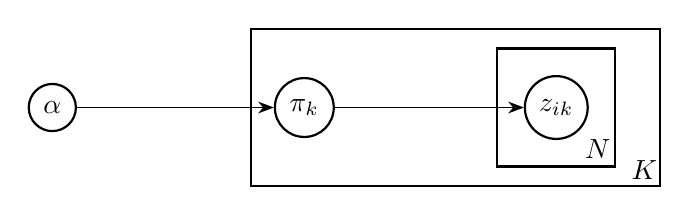
\begin{tikzpicture} [scale = 1.6] 
        %style
        \tikzset{circle/.style = {shape=circle, draw ,minimum size=1.5em, text opacity=1, thick}}
        \tikzset{quad/.style = {shape=rectangle, draw, minimum size=1.5,text opacity=1, thick, minimum width = 1.5cm, minimum height = 1.5cm}}
        \tikzset{rectangle/.style = {shape=rectangle, draw, minimum size=1.5,text opacity=1, thick, minimum width = 5.2cm, minimum height = 2.0cm}}
        \node[circle]    (alpha) at  (0,0) {$\alpha$};
        \node[circle]    (theta) at  (2,0) {$\pi_k$};
        \node[circle]    (zeta)  at  (4,0) {$z_{ik}$};
        \node[quad] (quad)  at  (4,0) {};
        \node[rectangle] (rect)  at  (3.2,0) {};
        \node            (N)     at  (4.33,-0.33) {$N$};
        \node            (K)     at  (4.70,-0.50) {$K$};
        \draw [-{Stealth[length=2mm]}] (alpha) to (theta);
        \draw [-{Stealth[length=2mm]}] (theta) to (zeta);
\end{tikzpicture}
\caption{Graphical model for the beta-binomial model}
\label{fig:beta-binomial}
\end{center}
\end{figure}
\end{frame}
%---------------------------------------------------------------------------------------
\begin{frame}{Finite Feature Model}
\setlength{\leftmargini}{0.2cm}
\begin{itemize}
\item Integrating over all values of $\vecpi$,  the probability of a binary matrix $\matz$ is
\begin{align}
    P(\matz) &= \prod_{k=1}^{K} \int  \bigg( \prod_{i=1}^{N}P(z_{ik}| \, \pi_k)\bigg)p(\pi_k) \diff \pi_k \nonumber \\
    &= \prod_{k=1}^{K} \frac{B(m_k + \aOverK, N-m_k+1)}{B(\aOverK,1)} \nonumber \\
    &= \prod_{k=1}^{K} \frac{\aOverK\Gamma(m_k+\aOverK)\Gamma(N-m_k+1)}{\Gamma(N+1+\aOverK)}, \label{eq:finiteFeature}
\end{align}
the result follows from the beta-binomial conjugacy and the distribution is  \textbf{exchangeable}, depending only on the counts $m_k$.
\end{itemize}
\end{frame}
%---------------------------------------------------------------------------------------
\begin{frame}{Equivalence Classes: Left-Ordered Matrices}
\setlength{\leftmargini}{0.2cm}
\begin{itemize}
\item In order to use the same approach as before and letting $\rightarrow\infty$ we need to define \textbf{equivalence classes of binary matrices}.
\item Let $lof( \cdot)$ a \textbf{many-to-one function ordering the columns of the binary matrix} $\matz$ from left to right by the magnitude of the binary number expressed by that column.
\item We denote by  $[\matz]$ the $lof$-equivalence class of a binary matrix $\matz$, i.e. 
\begin{equation*}
    [\matz] = \{ \boldsymbol{Y}: lof(\boldsymbol{Y})=lof(\matz)\}.
\end{equation*}
\end{itemize}
\begin{figure}
    \centering
    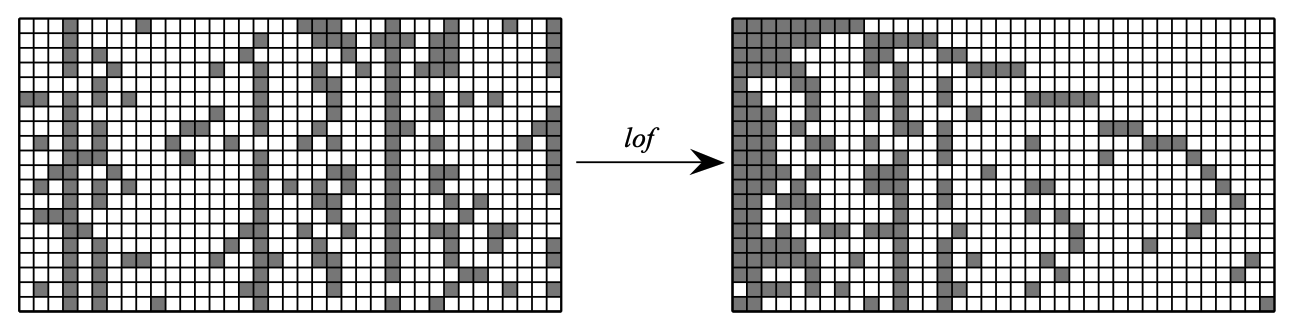
\includegraphics[width=0.7\columnwidth]{utilities/lof.png}
    \caption{$\matz$ and $lof(\matz)$}
    \label{fig:my_label}
\end{figure}
\end{frame}
%---------------------------------------------------------------------------------------
\subsection{Infinite Feature Model}
\begin{frame}{Infinite Feature Model}
\setlength{\leftmargini}{0.2cm}
\vspace{-5pt}
\begin{itemize}
\item From Equation \ref{fig:beta-binomial}, the probability of a particular $lof$-equivalence class is
\begin{align}
    P([\matz]) &= \sum_{\matz \in [\matz]} P(\matz) \nonumber\\
    &= \frac{K!}{\prod_{h=0}{2^N-1}K_h!} P(\matz), \label{eq:lofeq}
\end{align}
\item Substituting and rearranging Equation \ref{eq:finiteFeature} in Equation \ref{eq:lofeq} and letting $K\rightarrow \infty$
\begin{equation}
    P([\matz]) = \frac{\alpha^{K_+}}{\prod_{h=1}^{2^N-1}K_h!} \exp\{-\alpha H_N\} \prod_{k=1}^{K_+}\frac{(N-m_k)!(m_k-1)!}{N!}, \label{eq:infFeat}
\end{equation}
where $H_N=\sum_{j=1}^{N}\frac{1}{j}$.
\item The distribution is \textbf{exchangeable} and it is coherent with the prior distribution defined by \cite{Hjort_1990} and the stick breaking construction suggested in \cite{hjort_2007}.
\end{itemize}
\end{frame}
%---------------------------------------------------------------------------------------
\subsection{The Indian Buffet Process}
\begin{frame}{The Indian Buffet Process}
\setlength{\leftmargini}{0.2cm}
\begin{itemize}
\item The first customer starts at the left of the buffet and takes Poisson($\alpha$) number of dishes.
\item Customer $i$th moves along the buffet and takes dish $k$  with probability $\frac{m_k}{i}$ and then tries Poisson($\frac{\alpha}{i}$)  number of new dishes.
\end{itemize}
\onslide<2->{
\begin{figure}
\begin{center} 
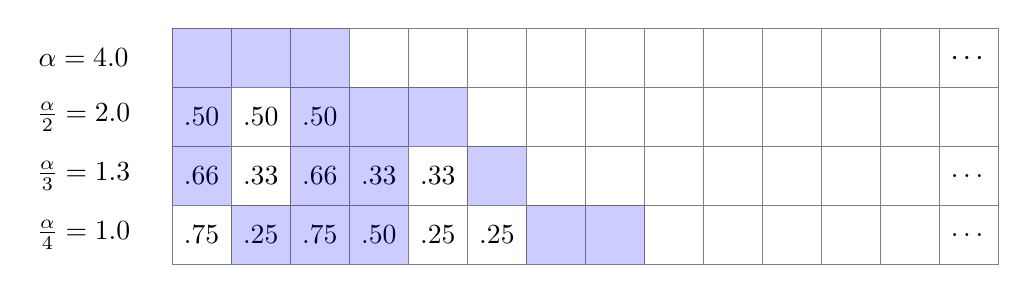
\begin{tikzpicture} [scale = 1.5]
    \draw[opacity=0.0] (-1.00,+0.50) rectangle (+6.0,-1.50);
    \draw[step=0.5cm,color=gray] (-1.00,+0.50) grid (+6,0,+0.00);
    \node at (+5.75,+0.25) {$\dots$};
    \fill[blue, opacity=0.2] (-1.00,+0.50) rectangle (-0.50,+0.00);
    \fill[blue, opacity=0.2] (-0.50,+0.50) rectangle (0.00,+0.00);
    \fill[blue, opacity=0.2] (-0.00,+0.50) rectangle (0.50,+0.00);
    \node at (-1.75,+0.25) {$\alpha =4.0$};
    
    \onslide<3>{
    \draw[step=0.5cm,color=gray] (-1.00,+0.00) grid (0.50,-0.50);
    \node at (-0.75,-0.25) {$.50$};
    \node at (-0.25,-0.25) {$.50$};
    \node at (+0.25,-0.25) {$.50$};
    }
    \onslide<4->{
    \draw[step=0.5cm,color=gray] (-1.00,+0.00) grid (+6.0,-0.50);
    \fill[blue, opacity=0.2] (-1.00,+0.00) rectangle (-0.50,-0.50);
    \fill[blue, opacity=0.2] (-0.00,+0.00) rectangle (0.50,-0.50);
    \fill[blue, opacity=0.2] (+0.50,+0.00) rectangle (1.00,-0.50);
    \fill[blue, opacity=0.2] (1.00,+0.00) rectangle (1.50,-0.50);
    \node at (+5.75,+0.25) {$\dots$};
    \node at (-1.75,-0.25) {$\frac{\alpha}{2} =2.0$};
    }
    \onslide<5>{
    \draw[step=0.5cm,color=gray] (-1.00,-0.50) grid (1.50,-1.00);
    \node at (-0.75,-0.75) {$.66$};
    \node at (-0.25,-0.75) {$.33$};
    \node at (+0.25,-0.75) {$.66$};
    \node at (+0.75,-0.75) {$.33$};
    \node at (+1.25,-0.75) {$.33$};
    }
    \onslide<6->{
    \draw[step=0.5cm,color=gray] (-1.00,-0.50) grid (+6.0,-1.00);
    \node at (+5.75,-0.75) {$\dots$};
    \fill[blue, opacity=0.2] (-1.00,-0.50) rectangle (-0.50,-1.00);
    \fill[blue, opacity=0.2] (-0.00,-0.50) rectangle (0.50,-1.00);
    \fill[blue, opacity=0.2] (+0.50,-0.50) rectangle (1.00,-1.00);
    \fill[blue, opacity=0.2] (+1.50,-0.50) rectangle (2.00,-1.00);
    \node at (-1.75,-0.75) {$\frac{\alpha}{3} =1.3$};
    }
    \onslide<7>{
    \draw[step=0.5cm,color=gray] (-1.00,-1.00) grid (2.00,-1.50);
    \node at (-0.75,-1.25) {$.75$};
    \node at (-0.25,-1.25) {$.25$};
    \node at (+0.25,-1.25) {$.75$};
    \node at (+0.75,-1.25) {$.50$};
    \node at (+1.25,-1.25) {$.25$};
    \node at (+1.75,-1.25) {$.25$};
    }
    \onslide<8->{
    \draw[step=0.5cm,color=gray] (-1.00,-1.00) grid (+6.0,-1.50);
    \node at (+5.75,-1.25) {$\dots$};
    \fill[blue, opacity=0.2] (-0.50,-1.00) rectangle (0.00,-1.50);
    \fill[blue, opacity=0.2] (-0.00,-1.00) rectangle (0.50,-1.50);
    \fill[blue, opacity=0.2] (+0.50,-1.00) rectangle (1.00,-1.50);
    \fill[blue, opacity=0.2] (+2.00,-1.00) rectangle (2.50,-1.50);
    \fill[blue, opacity=0.2] (+2.50,-1.00) rectangle (3.00,-1.50);
    \node at (-1.75,-1.25) {$\frac{\alpha}{4} =1.0$};
    }
\end{tikzpicture}
\caption{Example of Indian Buffet Process with $\alpha=4$}
\label{fig:IBP}
\end{center}
\end{figure}
}
\end{frame}
%---------------------------------------------------------------------------------------
\begin{frame}{IBP Properties}
\setlength{\leftmargini}{0.2cm}
\begin{itemize}
\item The previous IBP is not exchangeable! The number of new dishes depends on $i$. 
\item \textbf{Exchangeable IBP} is a generative process for distributions over collections of histories equivalent to $P([\matz])$ in Equation \ref{eq:infFeat}.
\item History of feature $k$ at object $i$ is defined to be $(z_{1k},\dots,z_{(i-1)k})$.
\begin{align*}
    e.g. \quad &(z_{1k}, z_{1k}) = (0, 0) \quad \quad\\
    &(z_{1k}, z_{2k}) = (1, 0)\\
    &(z_{1k}, z_{2k}) = (0, 1)\\
    &(z_{1k}, z_{2k}) = (1, 1)
\end{align*}
\end{itemize}
\setlength{\leftmargini}{0.4cm}
\begin{enumerate}
\item The effective dimension, $K_+$, of the model follows a Poisson($\alpha H_N$) distribution.
\item The number of features possessed by each object follows a Poisson($\alpha$)  distribution.
\item The expected number of entries in $\matz$ is $N\alpha$, so $\matz$ remains sparse as $K \rightarrow \infty$.
\end{enumerate}
\end{frame}
%---------------------------------------------------------------------------------------
\subsection{Gibbs Sampler}
\begin{frame}{Inference by Gibbs Sampling}
\setlength{\leftmargini}{0.2cm}
\begin{itemize}
\item To sample from the distribution defined by the IBP we need to compute the full conditional $P(z_{ik}=1 | \, \matz_{-(ik)})$, where $\matz_{-(ik)}$ denotes the entries of $\matz$ other than $z_{ik}$.
\item In the finite model, we use Equation \ref{eq:finiteFeature} for $P(\matz)$ to obtain the conditional distribution for any $z_{ik}$. Integrating out $\pi_k$
\begin{align*}
    P(z_{ik}=1|\, \vecz_{-i,k}) &= \int_{0}^{1}P(z_{ik}|\pi_k)p(\pi_k|\vecz_{-i,k}) \diff \pi_k \\ &=\frac{m_{-i,k}+\aOverK}{N+\aOverK}
\end{align*}
where $m_{-i,k}$  is the number of object with features $k$, not including $i$.
\item For the infinite case, \textbf{we arbitrary choose object \textit{i}th to be the last one to visit the buffet}
\begin{equation}
    P(z_{ik}=1|\, \vecz_{-i,k}) =\frac{m_{-i,k}}{N}, \label{eq:IBPGibbs}
\end{equation}
that is also the limit of the full conditional for the finite case.
\end{itemize}
\end{frame}
%---------------------------------------------------------------------------------------
\begin{frame}{IBP sampling algorithm}

\begin{algorithm}[H]
\begin{algorithmic}[1]
    \STATE Initialize binary matrix $\matz$
    \FOR{$i=1$ to $N$}
    \FOR{$k=i$ to $K$}
    \IF {$m_{-i,k}>0$}
    \STATE $z_{ik} \sim P(z_{ik}=1|\, \vecz_{-i,k})$
    \ELSE 
    \STATE Delete column $k$
    \ENDIF
    \STATE Add Poisson($\frac{\alpha}{N}$) new columns
    \ENDFOR
    \ENDFOR
    \end{algorithmic}
    \caption{Gibbs sampler for IBP}
    \label{alg:seq}
    \end{algorithm}
\end{frame}
%---------------------------------------------------------------------------------------
\subsection{Developments}
\begin{frame}{Two-Parameter IBP}
\setlength{\leftmargini}{0.2cm}
\begin{itemize}
\item IBP has only one parameter $ \alpha$ which controls both the \textbf{sparsity} of $\matz$ and its \textbf{dimensionality}.
\item \cite{Ghahramani_2007} introduced a a \textbf{two-parameter generalization of the IBP, with}
\begin{equation*}
    \pi_z | \, \alpha, \beta \sim \text{Beta}\Big(\frac{\alpha\beta}{K},\beta\Big)
\end{equation*}
\item The generative process
\end{itemize}
\setlength{\leftmargini}{0.6cm}
\begin{enumerate}
\item The first customer starts at the left of the buffet and samples Poisson($\alpha$) dishes. 
\item The $i$th customer takes any dish previously sampled with probability  $m_k/(\beta + i - 1)$, then he takes additional Poisson($\alpha\beta /(\beta +i-1$) dishes.
\end{enumerate}
\setlength{\leftmargini}{0.2cm}
\begin{itemize}
\item Parameter $\boldsymbol{\beta}$ \textbf{controls the  number of shared features} between objects.
\end{itemize}
\end{frame}
%---------------------------------------------------------------------------------------
\begin{frame}{Two-Parameter IBP}
\begin{figure}
    \centering\includegraphics[width=1\columnwidth]{utilities/two_parameters_IBP.png}
    \caption{ Three samples from the two-parameter IBP with $ \alpha = 10$ and $\beta = 0.2$ (left), $\beta = 1$ (middle), and $\beta = 5$ (right).}
    \label{fig:twoP_IBP}
\end{figure}
\end{frame}
%---------------------------------------------------------------------------------------
\section{Bibliography}
\begin{frame}[allowframebreaks]{Bibliography}
\bibliographystyle{abbrvnat}
\nocite{gr_gh_IBP_2011}
\bibliography{utilities/bibl.bib}
\end{frame}

%----------------------------------------------------------------------------------------

\end{document}











